\section{\textsc{BenchFill}：面向难度的缺口填补}

\begin{figure*}[t]
    \centering
    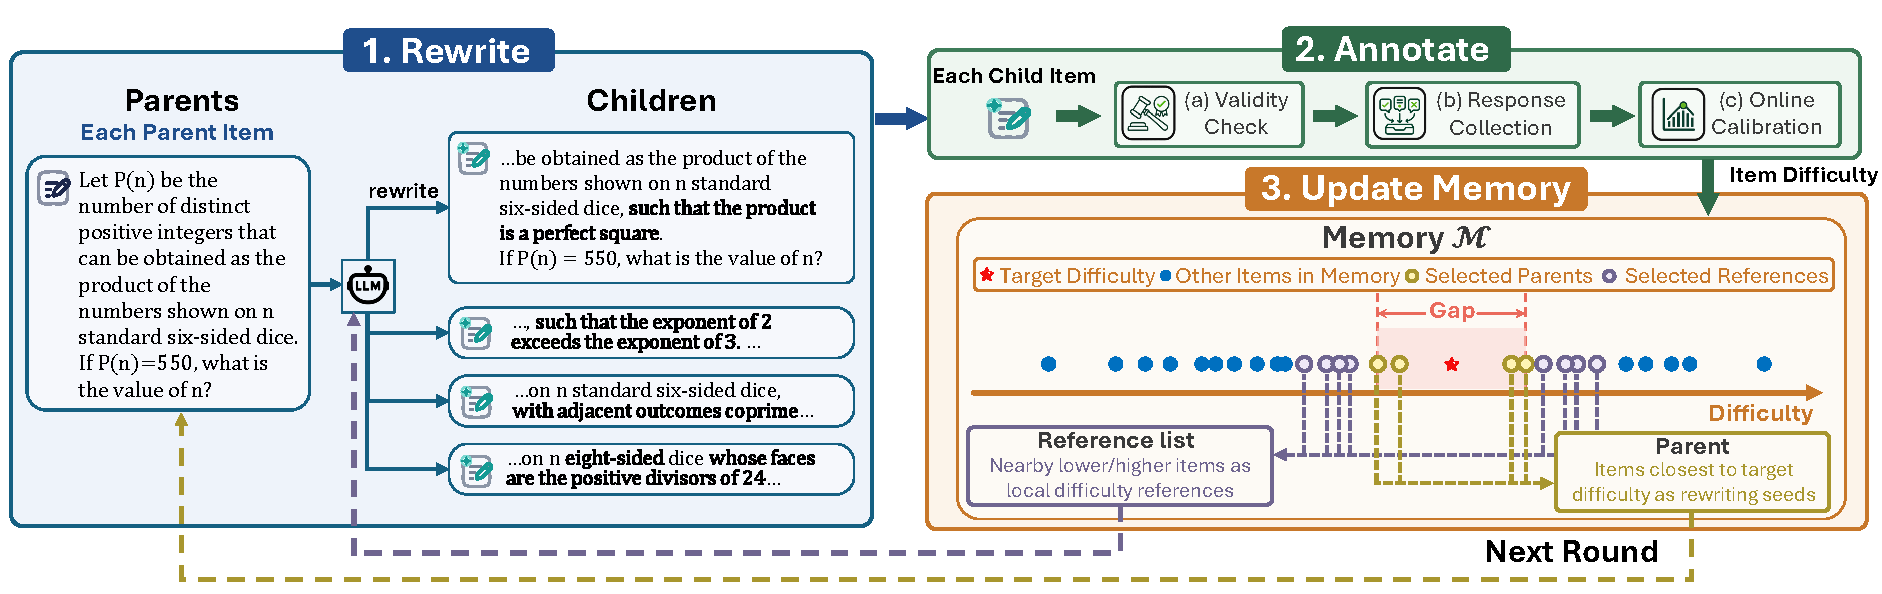
\includegraphics[width=\textwidth]{Fig/search.pdf}
      \vspace{-4mm}
    \caption{\textbf{\textsc{BenchFill} 概览。}
    \textsc{BenchFill} 迭代地将父题改写为子变体，标注其难度，并更新记忆以指导下一轮缺口填补。}
    \label{fig:benchfill_overview}
  \vspace{-4mm}
\end{figure*}

\subsection{问题设定与方法}

% As discussed above, large gaps in the difficulty distribution limit a benchmark's local resolution.
% By Theorem~\ref{thm:max-gap-detection-boundary}, reducing these gaps improves the benchmark's ability to capture localized model improvements. 
% As discussed above, reducing large gaps in the difficulty distribution improves a benchmark's local resolution and its ability to capture localized model improvements. In this section, we introduce \textsc{BenchFill}, a propose-and-annotate evolutionary search algorithm~\citep{sharma5openevolve,liu2026evox} for difficulty-targeted item rewriting. Rather than generating items from scratch, \textsc{BenchFill} iteratively rewrites existing benchmark items, estimates the difficulties of the rewritten variants, and stores the resulting item--difficulty pairs in a memory bank. This memory guides subsequent rewrites toward under-covered regions of the difficulty axis. The complete pseudocode is provided in Alg.~\ref{alg:gap_filling}.
% The algorithm proceeds iteratively. At each round, it proposes a set of candidate benchmark items, estimates their difficulties, and stores the resulting item--difficulty pairs in a memory bank for subsequent proposals. By conditioning new generations on previously observed item--difficulty pairs, the search gradually moves toward the target difficulty and produces items that effectively fill the identified gaps. 
% The complete pseudocode is provided in Alg.~\ref{alg:gap_filling}.

\paragraph{问题设定。}
令 $B=\{x_i\}_{i=1}^n$ 为当前基准，其中每道题 $x_i$ 具有估计难度 $z_i$。我们将难度排序，并考虑两道基准题之间的相邻间隔 $[z_L,z_R]$。缩小此类间隔可以提高基准的局部分辨率及其捕捉局部模型改进的能力。因此，我们的目标是得到一道有效的新题 $x_{\mathrm{new}}$，其难度尽可能接近目标难度 $z^\star=(z_L+z_R)/2$，即单次插入下最能缩小该间隔的中点。新题被加入基准，而不是替换任何已有题目。默认情况下，我们对该基准的\textit{最大}间隔应用这一过程。

一种直接做法是请人类专家按目标难度设计新题，但这一过程可能代价高昂~\cite{rein2024,phan2025humanity}。受近期关于 LLM 辅助基准扩充的工作启发~\cite{cheng2026vera,li2025ride,ying2024automating,xia2024top}，我们改为使用 LLM 将已有基准题\textit{改写}为针对目标难度的新变体。这种基于改写的方法可扩展，以已有题目作为局部参照来控制难度调整，并有助于保持原始基准的格式与风格。为确保题目质量，最终入选的题目还会由人类专家进一步验证。接下来我们介绍 \textsc{BenchFill}，一种用于自动、面向目标难度的题目改写的“改写并标注”进化搜索算法~\citep{sharma5openevolve,liu2026evox}。算法~\ref{alg:gap_filling} 给出伪代码，图~\ref{fig:benchfill_overview} 说明该过程。

\paragraph{\textsc{BenchFill}。}
给定目标难度 $z^\star$，算法维护一个由已标注题目--难度对组成的记忆 $\mathcal{M}$。记忆用难度最接近所选间隔的已有基准题初始化，并在搜索过程中更新。每一轮执行一步父--子改写。\emph{父题}是从 $\mathcal{M}$ 中选出、作为改写主要参照的已有题目或先前改写得到的题目，而\emph{子题}是由父题派生的新提议变体。


在第 $t$ 轮，我们从 $\mathcal{M}$ 中检索一小批标注难度最接近目标难度 $z^\star$ 的父题。对每个父题，改写 LLM 以该父题、目标难度以及附近题目--难度对的参照列表为条件。参照列表提供 $z^\star$ 附近的局部样例，通常包括略低于和略高于目标难度的题目，例如当 $z^\star=0.55$ 时，难度为 $0.48,0.50,0.60$ 与 $0.62$ 的题目。随后改写器将每个父题改写为一批子题，同时保持基准的格式与风格。


改写之后，每个子题被送入下文详述的难度标注模块，该模块返回估计难度 $\hat{z}$。我们只保留有效\footnote{我们使用 GPT-5.4 作为有效性评判器，核验每道改写题目所附答案是否正确。}的子题，并将其标注后的题目--难度对 $(x,\hat{z})$ 加回 $\mathcal{M}$。这一更新使搜索具有自适应性：每当某个改写子题比先前题目更接近 $z^\star$，它在后续轮次中就更可能被检索为父题或进入参照列表。因此，随着搜索推进，改写器以越来越与目标相关的样例为条件，而不是独立地改写每一批。经过 $T$ 轮后，我们选择使 $|\hat{z}-z^\star|$ 最小的有效子题作为提议的缺口填补题目。在插入基准之前，最终题目须经过人类专家的仔细人工审核。

\paragraph{难度标注模块的细节。}
对每道改写题目 $x$，我们在原始基准上拟合的 IRT 模型下，通过在线校准标注其难度。令 $\hat{\theta}_j$ 为模型 $j$ 预先估计的能力。我们对 $x$ 评估每个模型 $K_j$ 次试验，并观测到 $c_j$ 次正确回答。题目难度通过只拟合新题目参数来估计：
\[
\hat{b}(x)
=
\arg\max_b
\sum_{j=1}^{m}
\left[
c_j\log \sigma(\hat{\theta}_j-b)
+
\bigl(K_j-c_j\bigr)\log\bigl(1-\sigma(\hat{\theta}_j-b)\bigr)
\right],
\]
其中 $\sigma(\cdot)$ 为 logistic 函数\footnote{对选择题基准，我们额外纳入与原始 IRT 拟合相同的机会水平猜测参数，此处为记号简便而省略。}。这种在线校准把每道改写题目放到与原始基准相同的 IRT 标尺上，而无需重新拟合整个模型。




\subsection{实验设置与结果}

\paragraph{实验设置。}
我们在来自不同领域的 8 个代表性基准上进行缺口填补。对每个基准，我们针对三个最显著的覆盖缺口。我们使用 MiniMax-M2.7~\cite{chen2026minimax} 作为改写 LLM，temperature 设为 $1.0$。搜索最多进行 8 轮；每一轮检索 4 个父题，将每个父题改写为 4 个子题，并提供至多 16 个附近题目--难度对的参照列表。作为基线，我们使用预算匹配的 best-of-\(N\) 均匀父题改写变体。更多实现细节见附录~\ref{sec:app_gap}。

% \paragraph{Results.}
% % We evaluate the reduction in Top-5 Sum after gap filling.
% As shown in Tab.~\ref{tab:gap_filling_results}, with only three inserted items per benchmark, \textsc{BenchFill} reduces $\mathrm{Top\text{-}5\ Sum}$ by $18.11\%$--$27.71\%$. We also include the oracle result, but only as a reference upper bound, not as an implementable gap-filling method. The achieved reductions are close to this oracle reference. For example, on AIME25, the oracle reduction is $29.40\%$, while \textsc{BenchFill} achieves $27.71\%$ and the budget-matched uniform-parent baseline achieves only $15.90\%$. These reductions show that \textsc{BenchFill} improves coverage of the largest under-covered difficulty regions, which can strengthen a benchmark's ability to monitor localized training progress. We further report Target Dev. and \textsc{BenchFill} consistently achieves a Target Dev. below \(0.01\), indicating that the rewrite-and-annotate search can produce items close to the intended difficulty levels. Representative generated items are shown in Tab.~\ref{tab:gap_filling_examples}. We will release the gap-filling benchmark items to support future evaluation studies.

\paragraph{结果。}
如表~\ref{tab:gap_filling_results} 所示，每个基准仅插入三道题，\textsc{BenchFill} 就将 $\mathrm{Top\text{-}3\ Sum}$ 降低 $21.09\%$--$38.88\%$。我们也给出 oracle 结果，但仅作为参照上界，而不是可实施的缺口填补方法。所取得的降幅接近这一 oracle 参照：平均而言，\textsc{BenchFill} 达到 $32.67\%$ 的降幅，oracle 为 $35.06\%$，预算匹配的均匀父题基线为 $17.52\%$。在 AIME24、AIME25 与 AIME26 上，\textsc{BenchFill} 达到了 oracle 降幅。这些降幅表明，\textsc{BenchFill} 改善了最大未覆盖难度区域的覆盖，从而可以增强基准监测局部训练进展的能力。我们进一步报告目标偏差（Target Dev.），\textsc{BenchFill} 始终将 Target Dev. 控制在 \(0.01\) 以下，表明我们提出的算法能够产生接近预期难度水平的题目。有代表性的生成题目见表~\ref{tab:gap_filling_examples}。

\begin{table*}[!t]
\centering
\caption{\textbf{缺口填补结果。}
前 3 大间隔之和降幅报告相对于原始基准的相对降幅（\%），越大越好。Target Dev. 是三个被填补间隔上，所选题目难度与目标难度之间的平均绝对偏差，越低越好。基线使用预算匹配的 best-of-\(N\) 均匀父题改写策略。Oracle 是一个\textit{理想化上界}：它依次插入三道题，每道都位于当前最大间隔的中点，而不是一种实际的缺口填补方法。
}
\label{tab:gap_filling_results}
\small
\resizebox{0.8\textwidth}{!}{
\begin{tabular}{lccccc}
\toprule
\textbf{基准}
& \multicolumn{3}{c}{\textbf{前 3 大间隔之和降幅（\%）} $\uparrow$}
& \multicolumn{2}{c}{\textbf{Target Dev.} $\downarrow$} \\
\cmidrule(lr){2-4}
\cmidrule(lr){5-6}
& \textbf{基线} & \textbf{\textsc{BenchFill}} & \cellcolor{gray!15}\textbf{Oracle}
& \textbf{基线} & \textbf{\textsc{BenchFill}} \\
\midrule
AIME24 & 6.90 & 35.57 & \cellcolor{gray!15}{35.57} & 0.057 & 0.005 \\
AIME25 & 27.44 & 37.56 & \cellcolor{gray!15}{37.56} & 0.016 & 0.005 \\
AIME26 & 17.94 & 33.04 & \cellcolor{gray!15}{33.04} & 0.045 & 0.002 \\
AMC23 & 24.47 & 35.19 & \cellcolor{gray!15}{35.78} & 0.009 & 0.003 \\
Gaokao2023en & 11.45 & 38.88 & \cellcolor{gray!15}{45.47} & 0.152 & 0.004 \\
BBH-3 objects & 14.83 & 29.88 & \cellcolor{gray!15}{32.80} & 0.026 & 0.006 \\
MMLU-Pro-Biology & 22.23 & 30.13 & \cellcolor{gray!15}{36.84} & 0.046 & 0.006 \\
IFEval & 14.94 & 21.09 & \cellcolor{gray!15}{23.44} & 0.036 & 0.007 \\
\midrule
平均 & 17.52 & 32.67 & \cellcolor{gray!15}{35.06} & 0.048 & 0.005 \\
\bottomrule
\end{tabular}
}
    \vspace{-5mm}
\end{table*}

\begin{figure*}[!t]
    \centering
    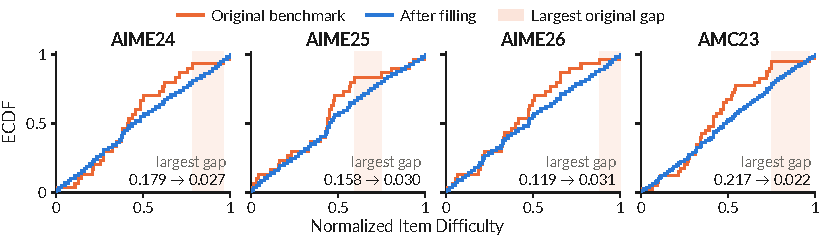
\includegraphics[width=\linewidth]{Fig/ecdf_paper.pdf}
      \vspace{-4mm}

    \caption{\textbf{四个基准在缺口填补前后的难度分布。} 橙色与蓝色曲线分别表示应用 \textsc{BenchFill} 之前与之后的经验难度分布。阴影区域标出原始的最大覆盖缺口。标注数值给出填补前后的最大间隔。}
    \label{fig:curated_benchmarks}
        \vspace{-5mm}
\end{figure*}

\subsection{经过整理的缺口填补基准}
\label{sec:curated_benchmarks}

为给未来模型与训练方法的更可靠评测提供社区资源，我们进一步将 \textsc{BenchFill} 应用于四个覆盖缺口显著、被广泛使用的数学基准，构造其缺口填补变体：AMC23、AIME24、AIME25 与 AIME26。我们将这些基准分别从 40、30、30 与 30 道题扩展到 80、50、52 与 53 道题。所有生成题目都经过人工审核，低质量或错误的题目被丢弃。我们将所得变体发布为 \textbf{AMC23-BenchFill}、\textbf{AIME24-BenchFill}、\textbf{AIME25-BenchFill} 与 \textbf{AIME26-BenchFill}\footnote{\url{https://huggingface.co/datasets/Yifan99/BenchFill}}。如图~\ref{fig:curated_benchmarks} 所示，这些变体大幅缩小了原始的最大覆盖缺口，并使经验难度分布更接近均匀分布，从而在难度谱上提供更全面的覆盖。


% \begin{table*}[t]
% \centering
% \caption{\textbf{Gap-filling results.}
% Target Dev. denotes the mean absolute deviation between the selected item difficulty and the target difficulty over three filled gaps. Top-5 Sum denotes the total size of the five largest adjacent difficulty gaps. Lower is better for both metrics.}
% \label{tab:gap_filling_results}
% \small

% \begin{minipage}[t]{0.49\linewidth}
% \vspace{0pt}
% \centering
% \resizebox{\linewidth}{!}{
% \begin{tabular}{lccccc}
% \toprule
% \textbf{Benchmark} 
% & \multicolumn{2}{c}{\textbf{Target Dev.} $\downarrow$}
% & \multicolumn{3}{c}{\textbf{Top-5 Sum} $\downarrow$} \\
% \cmidrule(lr){2-3}
% \cmidrule(lr){4-6}
% & \textbf{Rand.} & \textbf{\textsc{BenchFill}}
% & \textbf{Before} & \textbf{Rand.} & \textbf{\textsc{BenchFill}} \\
% \midrule
% AIME24 &  & 0.009 & 0.502 &  & 0.411 \\
% AIME25 &  & 0.007 & 0.492 &  & 0.355 \\
% AIME26 &  & 0.004 & 0.507 &  & 0.413 \\
% AMC23  &  & 0.005 & 0.528 &  & 0.397 \\
% \bottomrule
% \end{tabular}
% }
% \end{minipage}
% \hfill
% \begin{minipage}[t]{0.49\linewidth}
% \vspace{0pt}
% \centering
% \resizebox{\linewidth}{!}{
% \begin{tabular}{lccccc}
% \toprule
% \textbf{Benchmark} 
% & \multicolumn{2}{c}{\textbf{Target Dev.} $\downarrow$}
% & \multicolumn{3}{c}{\textbf{Top-5 Sum} $\downarrow$} \\
% \cmidrule(lr){2-3}
% \cmidrule(lr){4-6}
% & \textbf{Rand.} & \textbf{\textsc{BenchFill}}
% & \textbf{Before} & \textbf{Rand.} & \textbf{\textsc{BenchFill}} \\
% \midrule
% Gaokao2023en &  & 0.009 & 0.183 &  & 0.136 \\
% BBH-3 objects &  & 0.006 & 0.354 &  & 0.297 \\
% MMLU-Pro-Biology &  & 0.002 & 0.176 &  & 0.142 \\
% IFEval &  & 0.005 & 0.190 &  & 0.158 \\
% \bottomrule
% \end{tabular}
% }
% \end{minipage}

% \end{table*}
